\documentclass{article}
\usepackage[utf8]{inputenc}
\usepackage{hyperref}
\usepackage[letterpaper, portrait, margin=1in]{geometry}
\usepackage{enumitem}
\usepackage{amsmath}
\usepackage{booktabs}
\usepackage{graphicx}
\usepackage{mathtools}  
\usepackage{diffcoeff} 
\usepackage{hyperref}
\usepackage{physics}
\usepackage{adjustbox}
\hypersetup{
colorlinks=true,
    linkcolor=black,
    filecolor=black,      
    urlcolor=blue,
    citecolor=black,
}
\usepackage{natbib}

\usepackage{titlesec}
\usepackage{chngcntr}

\counterwithin*{equation}{section}
\counterwithin*{equation}{subsection}


  
\title{Homework 7}
\author{Economics 7103}
\date{Spring semester 2023}
  
\begin{document}

\maketitle
\section{}
See Fig.1.
\begin{figure}
    \centering
    \begin{adjustbox}{width=\textwidth}
    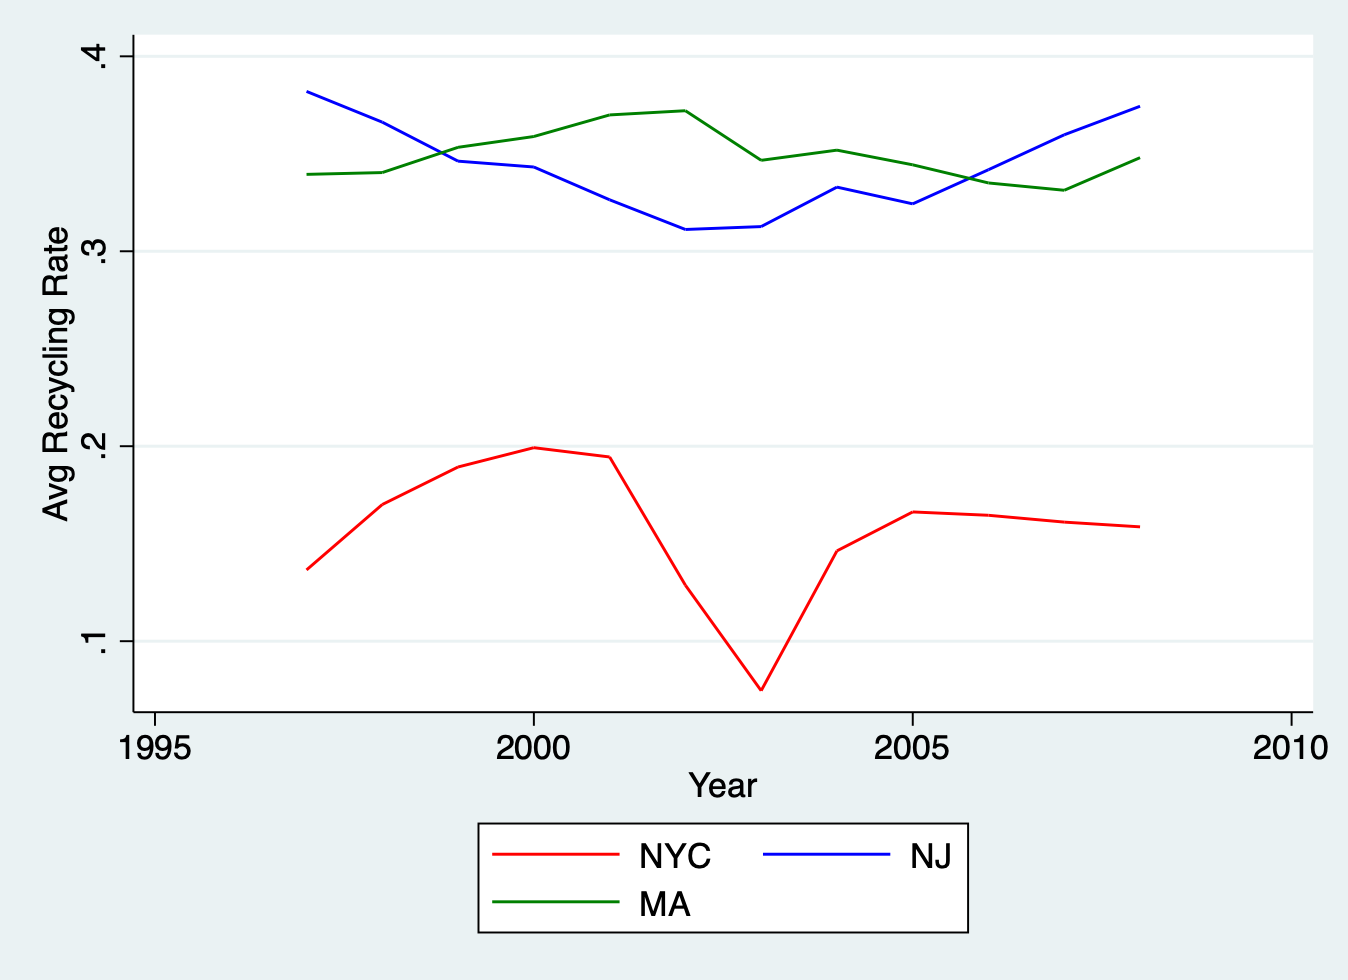
\includegraphics{Q1.png}
    \end{adjustbox}
    \caption{Recycling Rates}
    \label{fig:my_label}
\end{figure}

\section{}
The coefficient on treatment variable is -0.065. The robust standard error is 0.0013.


\section{}
See Fig.2.
\begin{figure}
    \centering
    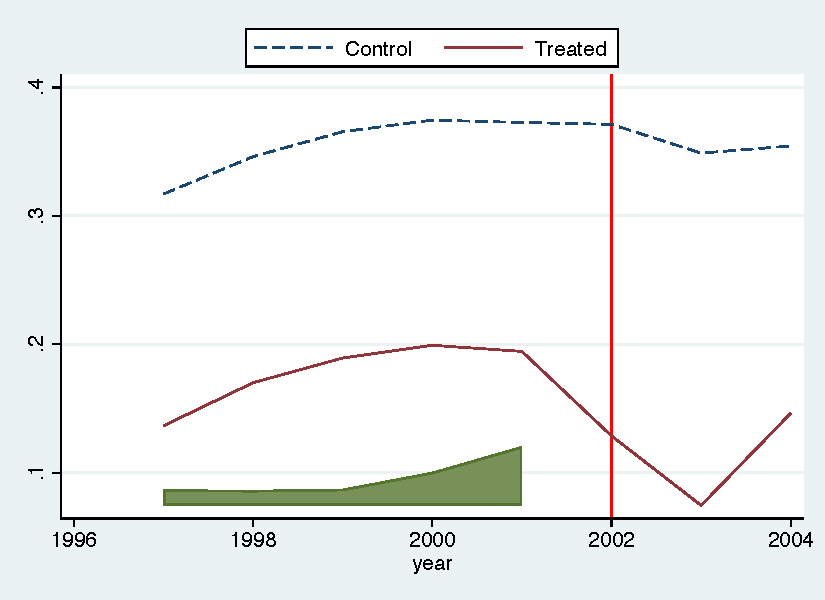
\includegraphics{Q3.pdf}
    \caption{Caption}
    \label{fig:my_label}
\end{figure}
\section{}
See Fig.3. 
\begin{figure}
    \centering
    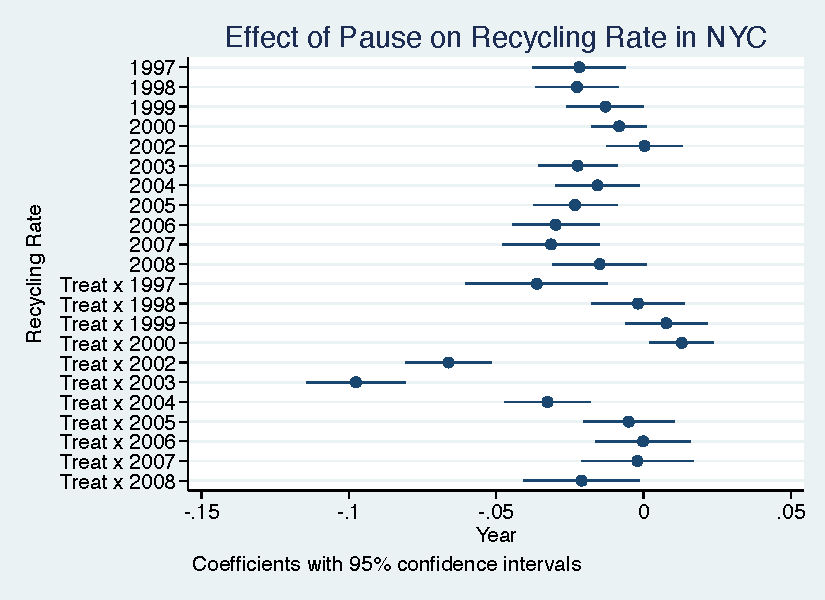
\includegraphics{Q4.pdf}
    \caption{Event Study}
    \label{fig:my_label}
\end{figure}
\section{}
\subsection{}
See Fig.4. 
\begin{figure}
    \centering
    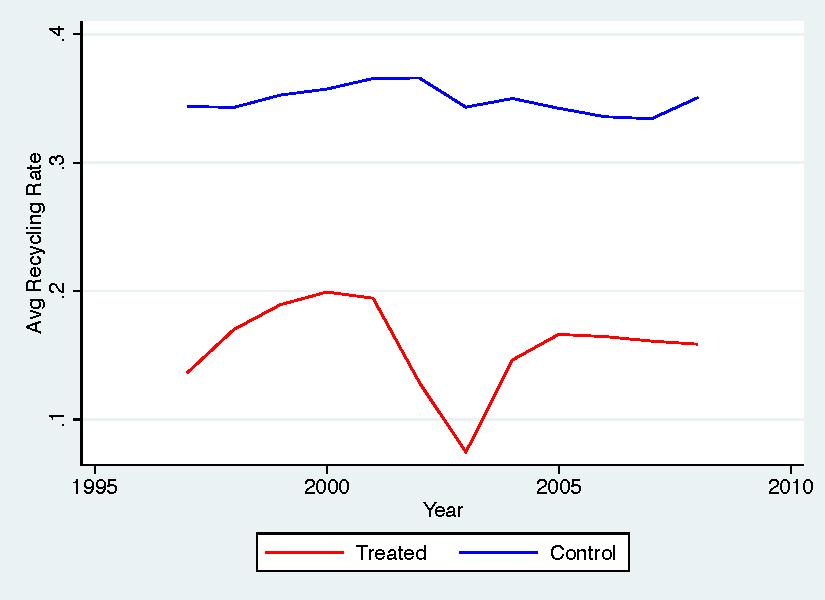
\includegraphics{5a.pdf}
    \caption{Treated vs Control}
    \label{fig:my_label}
\end{figure}


\subsection{}
See Fig.5.
\begin{figure}
    \centering
    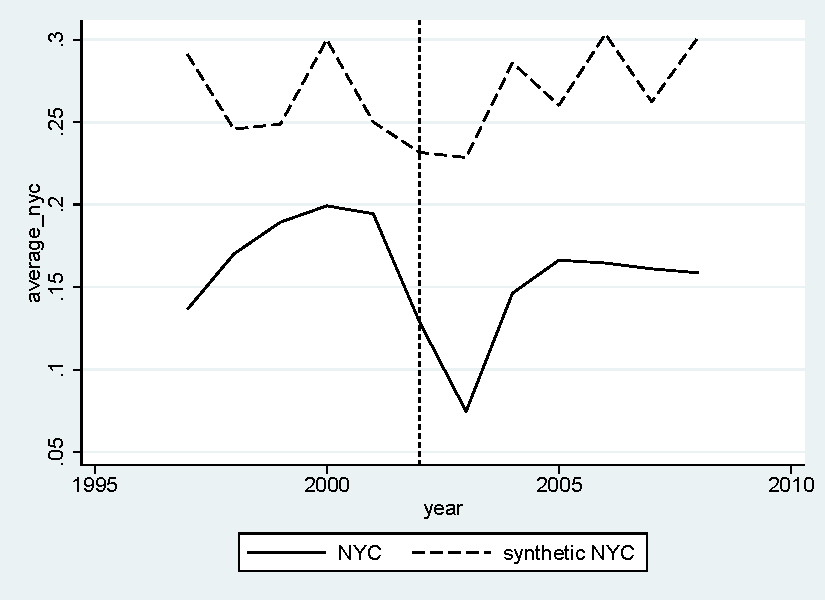
\includegraphics{5b.pdf}
    \caption{Synthetic control}
    \label{fig:my_label}
\end{figure}

\subsection{}
Code in the Stata file

\subsection{}
Taking L 


\end{document}
